\documentclass[mathserif]{beamer}

\usepackage{thesis}
\usepackage{pdfpages}
\usepackage{array}
\usepackage{booktabs}


\title[Sampling from Probabilistic Submodular Models]
{Sampling from Probabilistic Submodular Models}

\author[Alkis Gotovos]{}


\newcommand{\tab}[2]{%
\makebox[#1\linewidth][l]{#2}%
}

\begin{document}

\setbeamertemplate{background canvas}{}
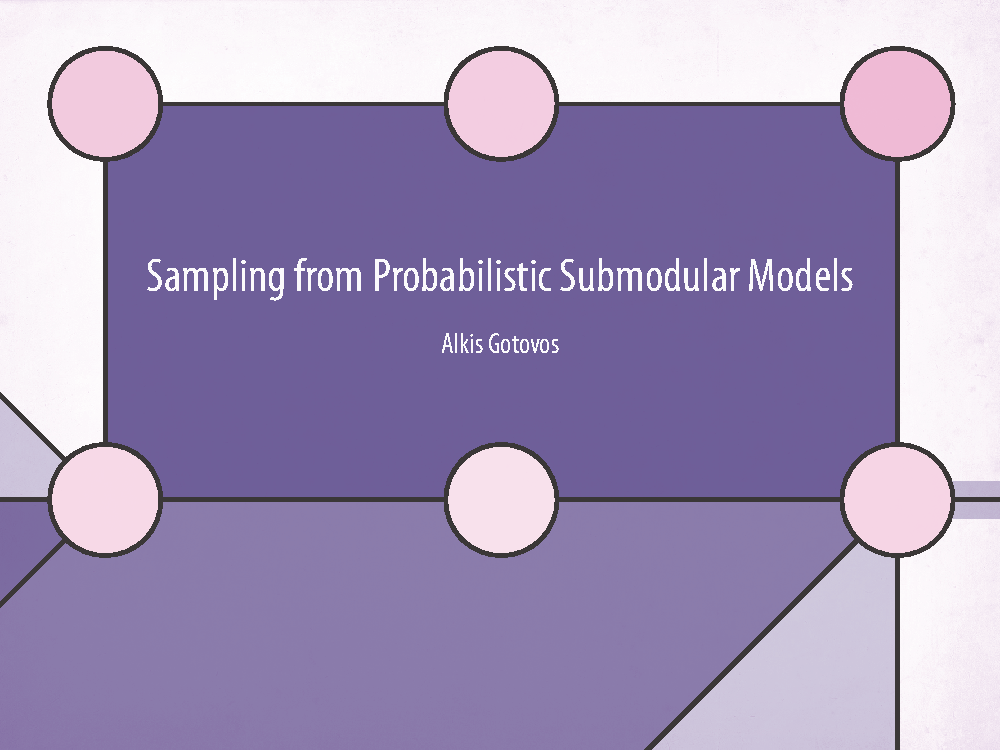
\includepdf[pages={1}]{title/title.pdf}
\setbeamertemplate{background canvas}{
\includegraphics[width=\paperwidth]{figures/bg_no_line.png}}


\begin{frame}{The Cancer Genome Atlas}
\vspace{0.5em}
\centering
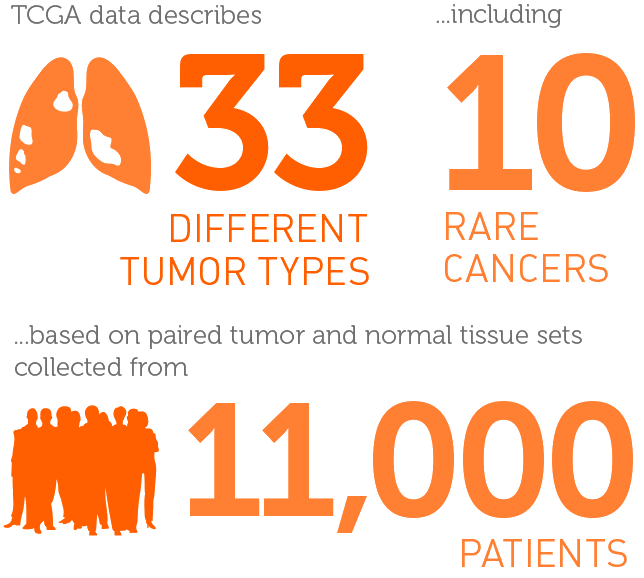
\includegraphics[width=2.5in]{figures/tcga.png}\\[-0.3em]
\hspace{12em}\qsource{cancergenome.nih.gov}
\end{frame}

\begin{frame}{The Cancer Genome Atlas}
\vspace{0.5em}
\centering
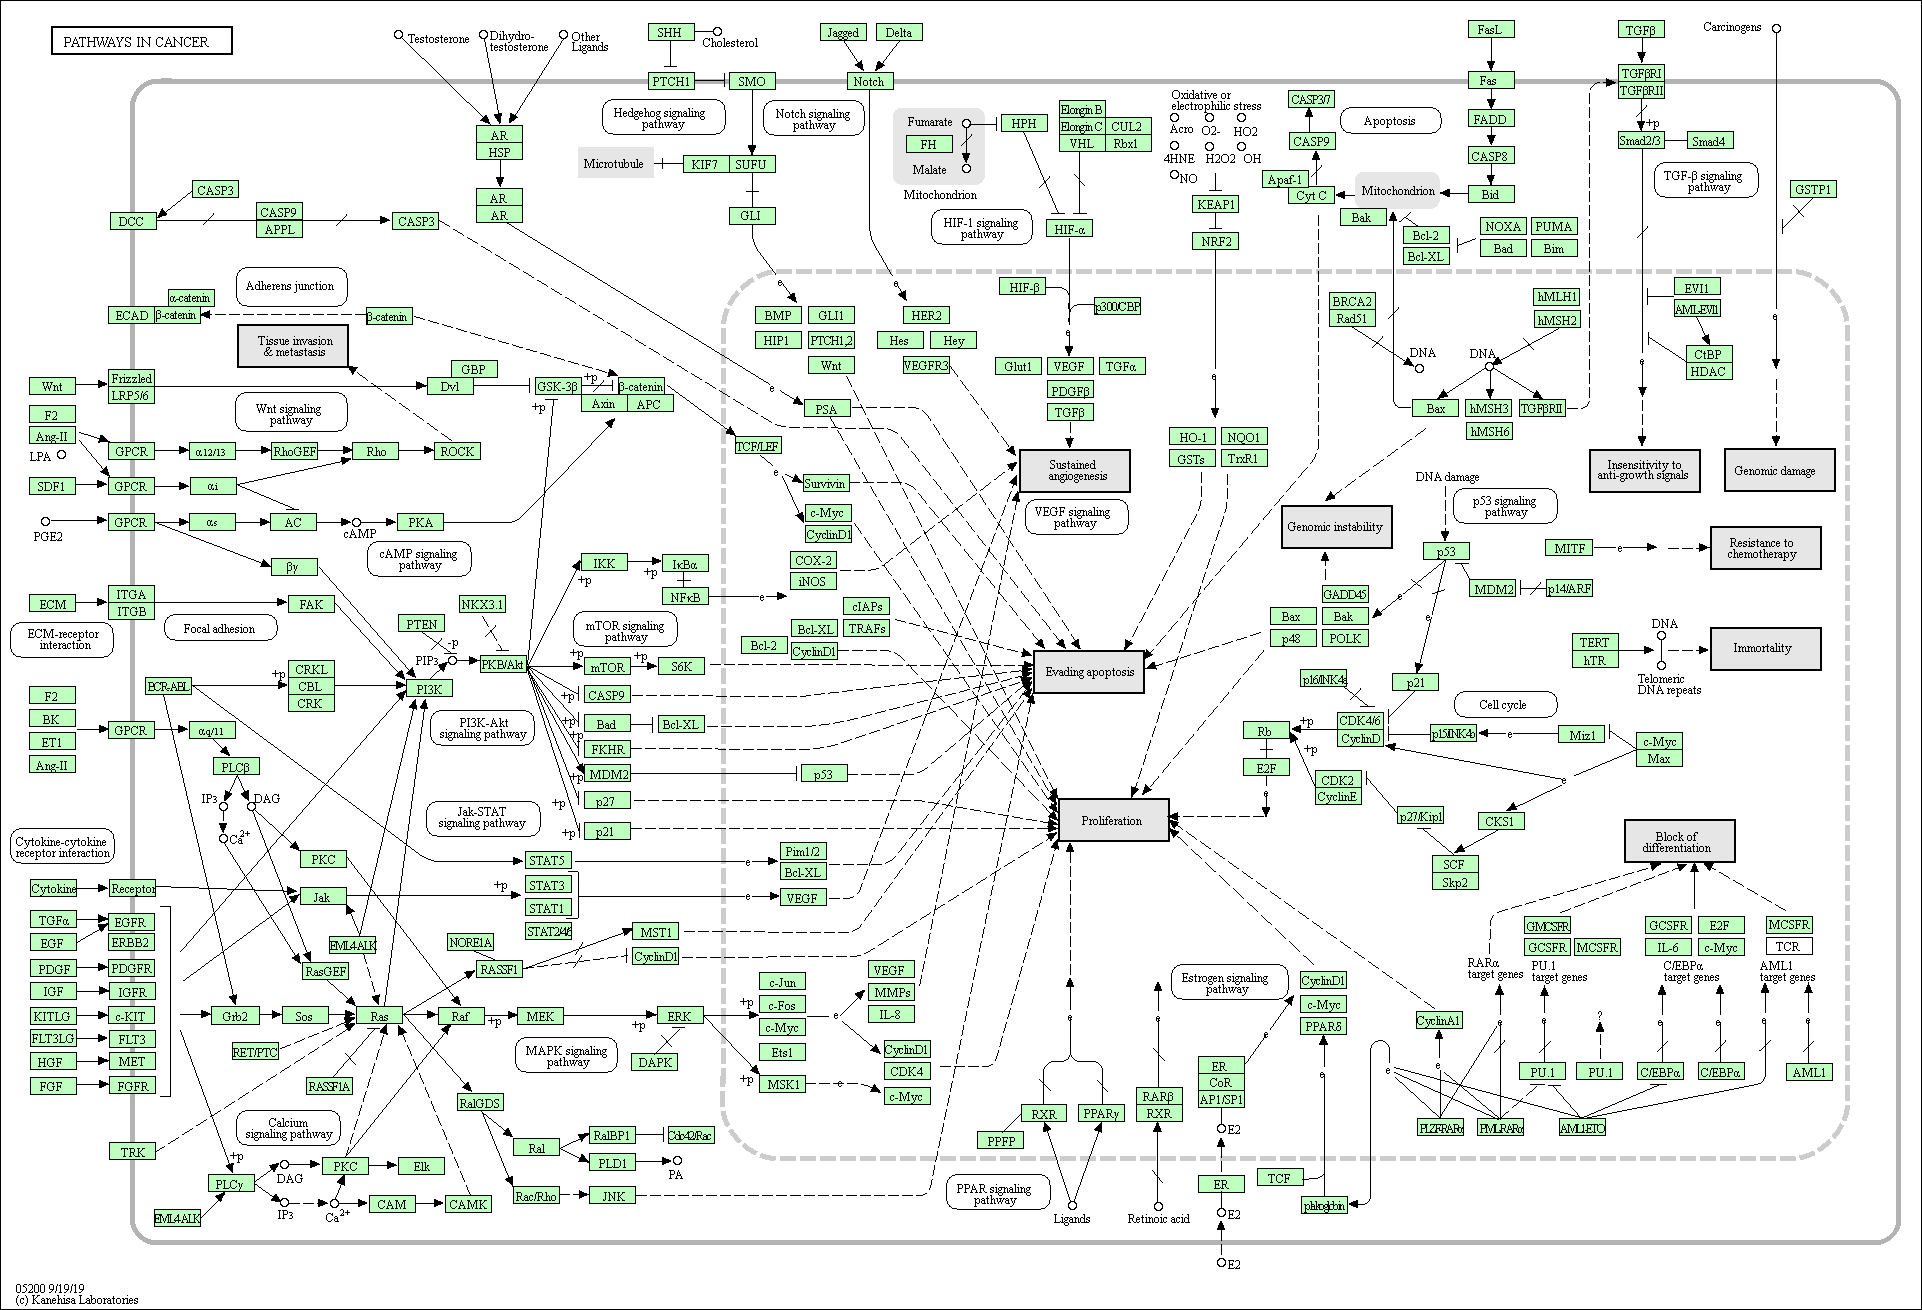
\includegraphics[width=\textwidth]{figures/pathways_alt.png}\\[-0.3em]
\hfill{}\qsource{genome.jp}
\end{frame}

\begin{frame}{Modeling Interactions between Gene Mutations}
\centering
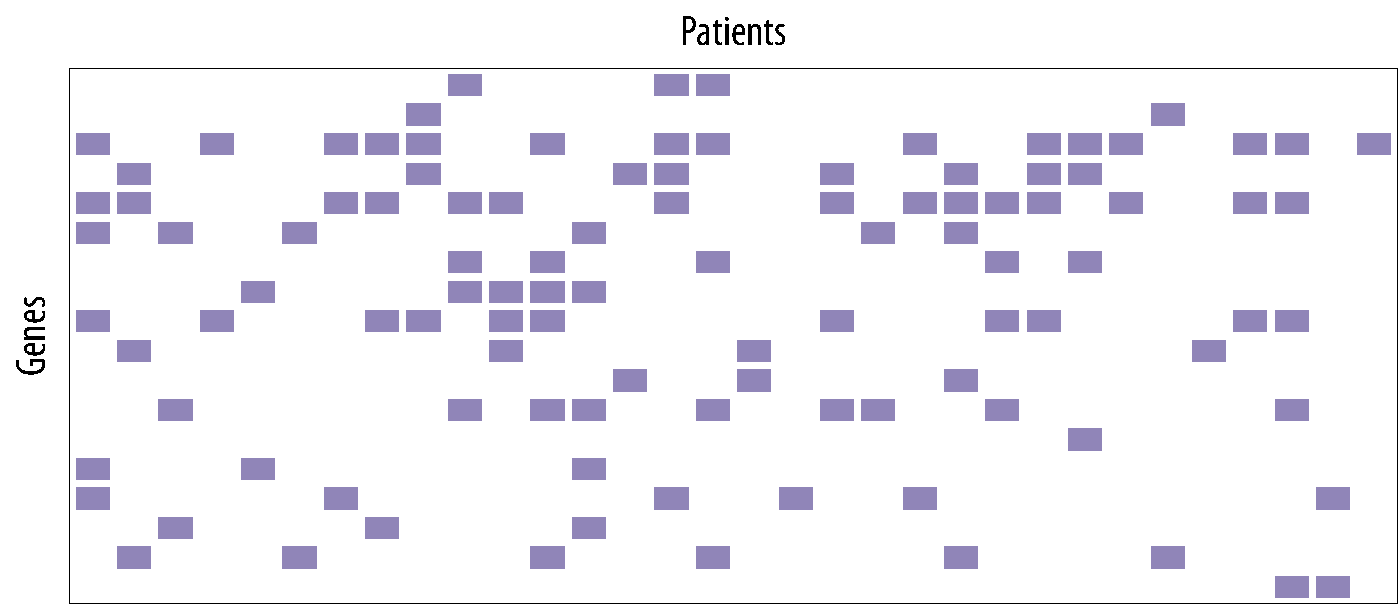
\includegraphics[width=3.7in]{figures/example1.pdf}
\end{frame}

\begin{frame}{Modeling Interactions between Gene Mutations}
\centering
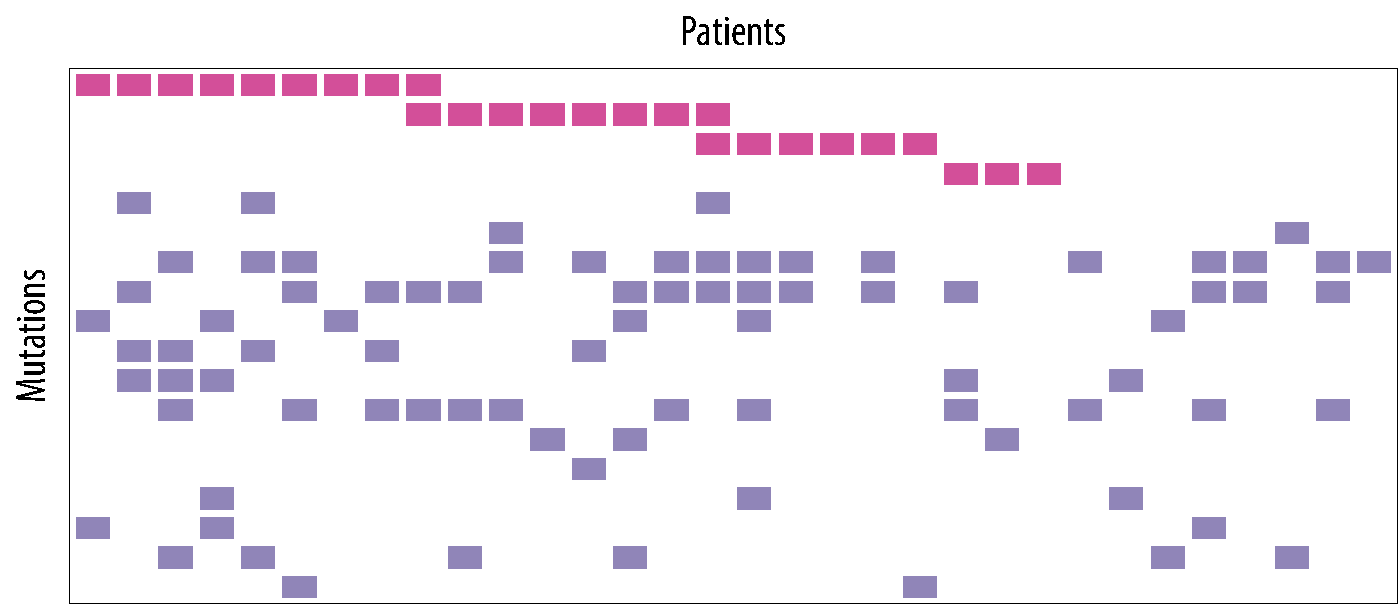
\includegraphics[width=3.7in]{figures/example1_rep.pdf}
\end{frame}

\begin{frame}{Modeling Interactions between Gene Mutations}
\centering
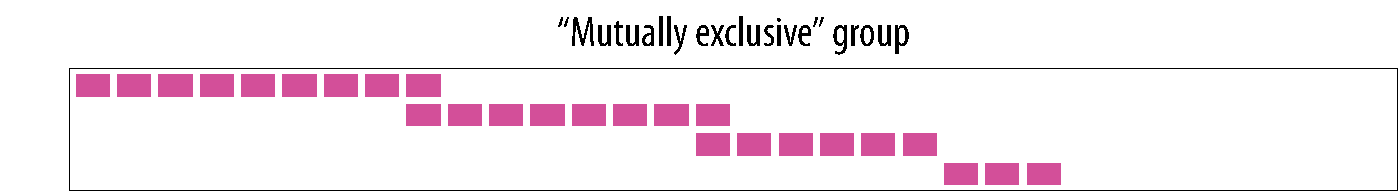
\includegraphics[width=3.7in]{figures/example1_rep_group.pdf}

\vspace{3em}

\begin{itemize}
\item<2-> \tab{0.4}{Discrete optimization \hspace{0.3em} 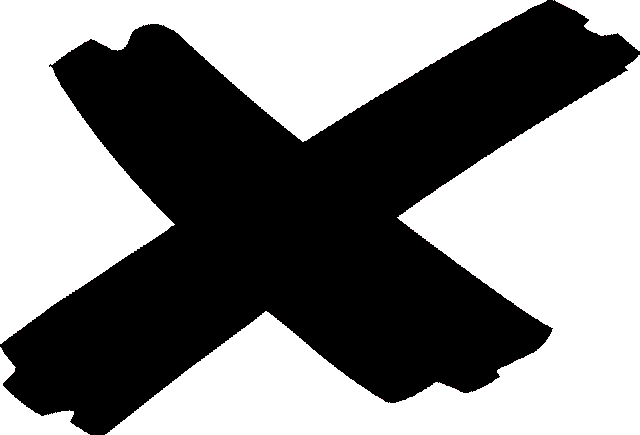
\includegraphics[width=0.13in]{figures/cross_mark.png}} \tab{0.15}{$\longrightarrow$} probabilistic models \hspace{0.3em} 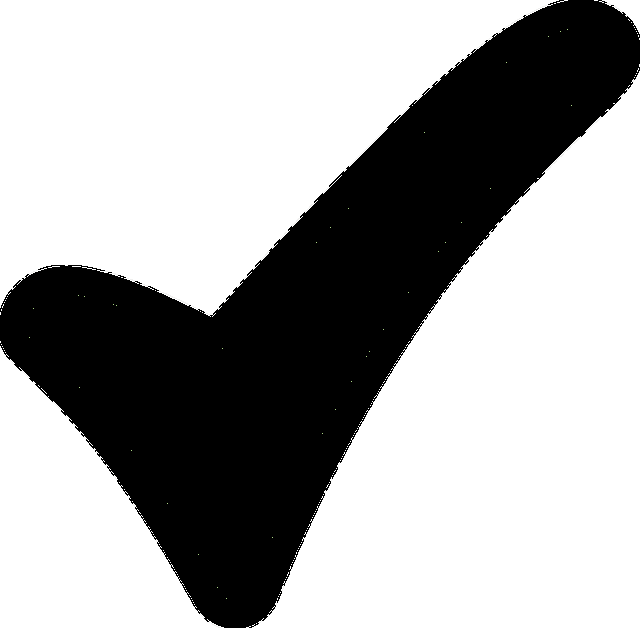
\includegraphics[width=0.13in]{figures/check_mark.png}
\vspace{0.7em}
\item<3-> \tab{0.4}{Classic pairwise models \hspace{0.3em} 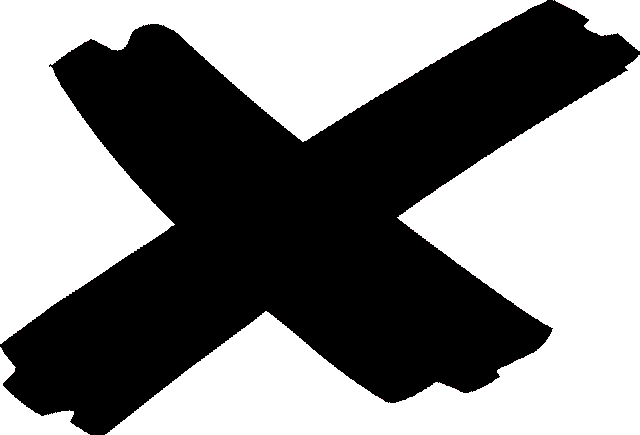
\includegraphics[width=0.13in]{figures/cross_mark.png}} \tab{0.15}{$\longrightarrow$} higher-order interactions \hspace{0.3em} 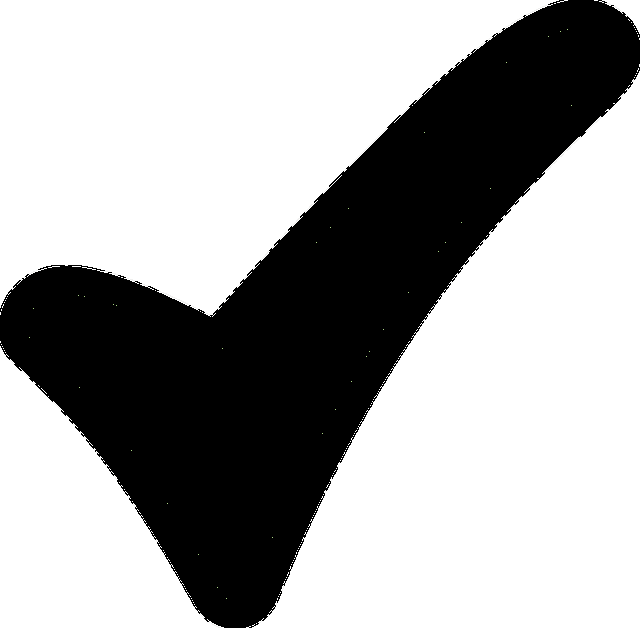
\includegraphics[width=0.13in]{figures/check_mark.png}
\vspace{0.7em}
\item<4-> \tab{0.4}{Deep nets \hspace{0.3em} 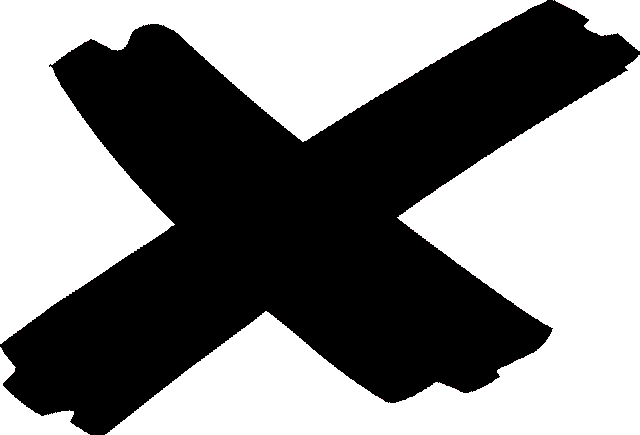
\includegraphics[width=0.13in]{figures/cross_mark.png}} \tab{0.15}{$\longrightarrow$} structured prior assumptions \hspace{0.3em} 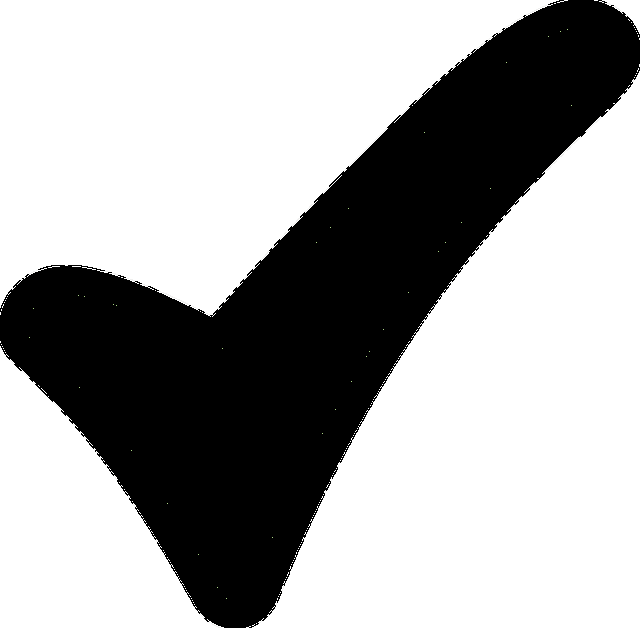
\includegraphics[width=0.13in]{figures/check_mark.png}
\end{itemize}
\end{frame}

\begin{frame}{Probabilistic Submodular Models}

\begin{center}
Distributions over subsets of $V = \{1,\ldots,n\}$

\vspace{0.8em}
\qboxa{
$p(S; \btheta) = \displaystyle\frac{1}{Z(\btheta)}\exp \big( F(S; \btheta) \big)$
}
\end{center}
\vspace{1.5em}

\begin{columns}
\begin{column}{0.54\textwidth}
\begin{itemize}
\item<2-> $F : 2^V \to \mathbb{R}\ $ is sub- or supermodular
\item<2-> $Z\ $ is the normalizer
\item<2-> $\btheta\ $ is a parameter vector
\end{itemize}
\vspace{0.6em}
\end{column}
\begin{column}{0.39\textwidth}
\uncover<3->{%
Well-studied subclasses
\begin{itemize}
\item Ising model (log-supermodular)
\item DPP (log-submodular)
\end{itemize}
}
\end{column}
\end{columns}

\end{frame}

\begin{frame}{Inference}
\vspace{1.75em}
\begin{center}
Distributions over subsets of $V = \{1,\ldots,n\}$

\vspace{0.8em}
\qboxa{
$p(S; \btheta) = \displaystyle\frac{1}{Z(\btheta)}\exp \big( F(S; \btheta) \big)$
}
\end{center}
\vspace{2em}

\uncover<2->{%
Fundamental tasks
}
\vspace{0.5em}
\hspace{11em}\tikzmark{right}
\begin{itemize}
\item<3-> Compute marginals $\ \mathbb{P}(a \in S \mid \{b, c\} \subseteq S)$ \tikzmark{i2}
\item<3-> Compute $\ Z$ \tikzmark{i3}
\item<5> Learn $\btheta$ from data
\end{itemize}

\uncover<4->{%
\begin{tikzpicture}[overlay, remember picture]
\node[anchor=base] (a) at (pic cs:i2) {\vphantom{h}}; % push the mark to the top of the line (ie including ascenders)
\node[anchor=base] (b) at (pic cs:i3) {\vphantom{g}}; % push the mark to the bottom of the line (ie including descenders)
\draw [decoration={brace,amplitude=0.5em},decorate,thick,col2]
 (a.north -| {pic cs:right}) -- (b.south -| {pic cs:right});
\node [text=col2,xshift=10.4em] (t) at ($(a)!0.5!(b)$) {\#P-hard in general};
\end{tikzpicture}
}

\end{frame}

\begin{frame}{Inference}
\vspace{0.5em}

\begin{minipage}{\textwidth}
\begin{columns}[c]
\column{0.36\textwidth}
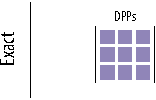
\includegraphics[height=0.7in]{figures/inf_dpp.pdf}
\column{0.57\textwidth}
\begin{itemize}
\item Tractable only for limited subclasses
\vspace{0.3em}
\item \#P-hard even for Ising models
\end{itemize}
\end{columns}
\end{minipage}

\uncover<2->{%
\vspace{2em}
\begin{minipage}{\textwidth}
\begin{columns}[c]
\column{0.36\textwidth}
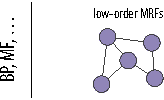
\includegraphics[height=0.7in]{figures/inf_mrf.pdf}
\column{0.57\textwidth}
\begin{itemize}
\item Extensively studied model class
\vspace{0.3em}
\item Complexity exponential in model order
\end{itemize}
\end{columns}
\end{minipage}
}

\uncover<3->{%
\vspace{2em}
\begin{minipage}{\textwidth}
\begin{columns}[c]
\column{0.36\textwidth}
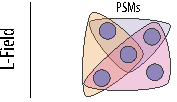
\includegraphics[height=0.7in]{figures/inf_psm.pdf}
\column{0.57\textwidth}
\begin{itemize}
\item Variational approach for general PSMs\\
\qcitea{Djolonga and Krause, 2014; Djolonga and Krause, 2015}
\end{itemize}
\end{columns}
\end{minipage}
}
\end{frame}

\begin{frame}{Thesis Topic}
\vspace{1em}
\centering
\only<1>{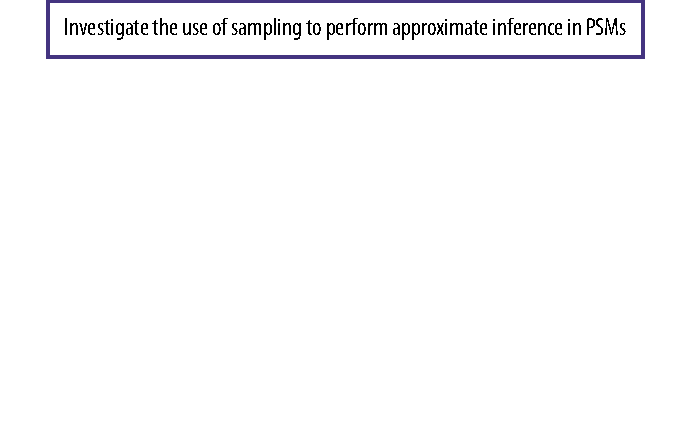
\includegraphics[width=\textwidth]{figures/chapters_topic.pdf}}%
\only<2>{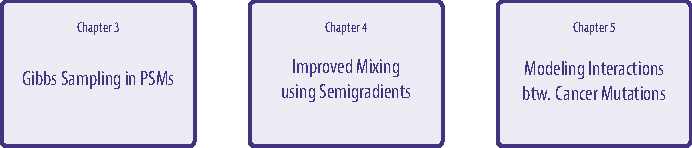
\includegraphics[width=\textwidth]{figures/chapters.pdf}}
\end{frame}

\begin{frame}{Gibbs Sampling in PSMs}
\vspace{1em}
\centering
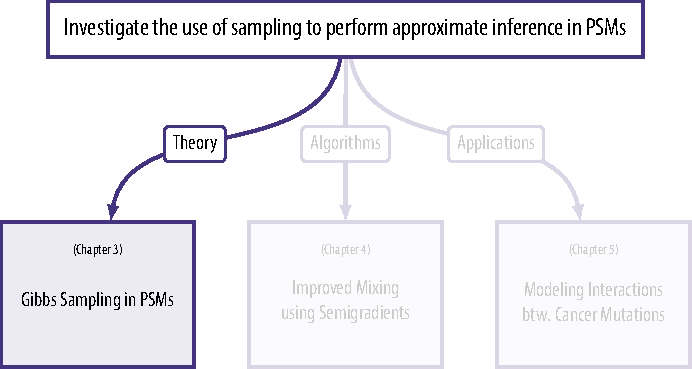
\includegraphics[width=\textwidth]{figures/chapters1.pdf}
\end{frame}

\begin{frame}{MCMC Sampling}
\begin{itemize}
\item Ground set $\ V = \{1,\ldots,n\}$
\item State space $\ \Omega = 2^V$
\item Transition matrix $\ P : \Omega \times \Omega \to \mathbb{R}$
\end{itemize}

%\vspace{1em}
\begin{center}
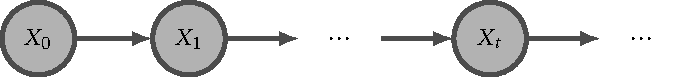
\includegraphics[width=3.3in]{figures/markov.pdf}
\end{center}

\vspace{1em}
\uncover<2->{%
Distance from stationarity $\ \ d(t) \defeq \max \left\{\|\mathbb{P}_{X_t} - p\|_{\textrm{tv}} \mid X_0 \in \Omega\right\}$}\\[1.5em]
\uncover<3->{Under mild conditions, $\ \ d(t) \xrightarrow{\ t\,\rightarrow\,\infty\ } 0\ \ \ \ $}\uncover<4->{{\color{col2} how fast?}}\\[1.6em]
\uncover<5->{Mixing time $\ \ t_{\textrm{mix}}(\epsilon) = \min \left\{t \mid d(t) \leq \epsilon \right\}$}
\end{frame}

\begin{frame}{The Gibbs Sampler}
\vspace{1em}
\centering
\only<1>{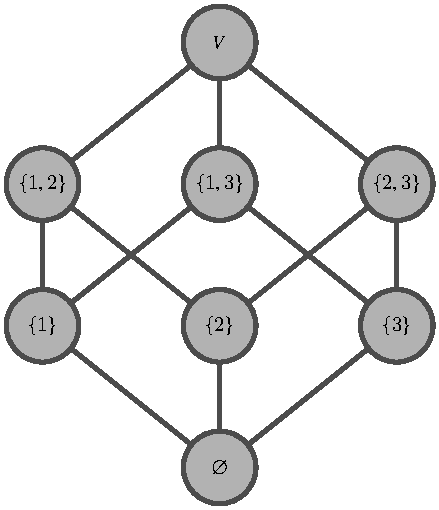
\includegraphics[width=2.5in]{figures/lattice_gibbs_0.pdf}}%
\only<2>{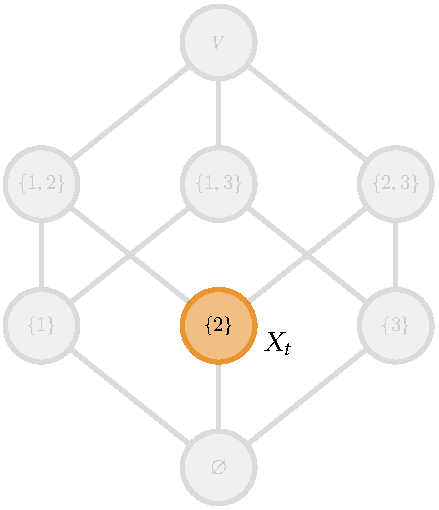
\includegraphics[width=2.5in]{figures/lattice_gibbs_1.pdf}}%
\only<3>{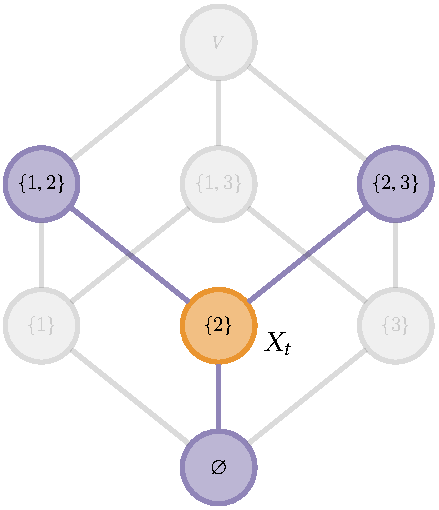
\includegraphics[width=2.5in]{figures/lattice_gibbs_2.pdf}}%
\only<4>{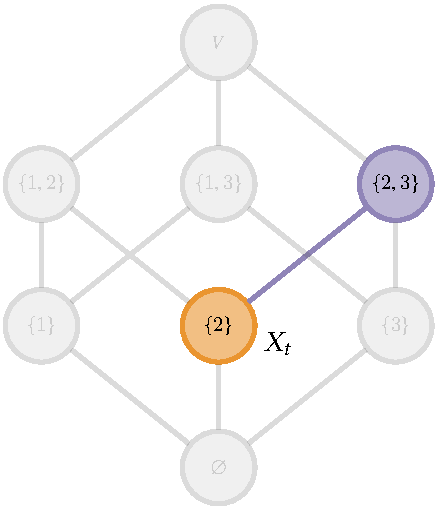
\includegraphics[width=2.5in]{figures/lattice_gibbs_3.pdf}}%
\end{frame}

\begin{frame}{The Gibbs Sampler}
\begin{center}
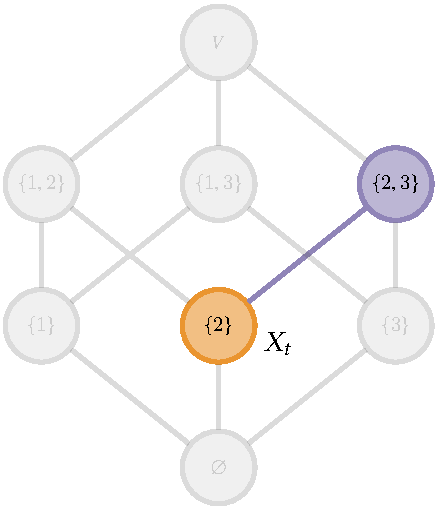
\includegraphics[width=1.4in]{figures/lattice_gibbs_3.pdf}
\end{center}

\centering
Mixing times are in general exponential in $|V|$ \qcitea{Jerrum and Sinclair, 1993}

\vspace{1em}
\centering
\qboxa{\minibox{We establish sufficient conditions for sub-exponential mixing\\of the Gibbs sampler on PSMs.}}
\end{frame}

\begin{frame}{Polynomial-time Mixing}
\vspace{0.5em}
\only<1>{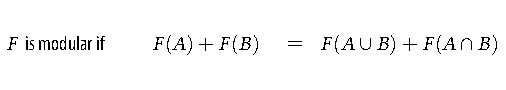
\includegraphics[width=3.9in]{figures/ineq_mod_0.pdf}}%
\only<2>{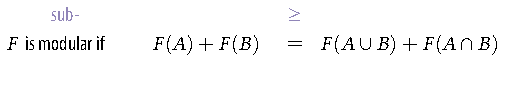
\includegraphics[width=3.9in]{figures/ineq_mod_1.pdf}}%
\only<3->{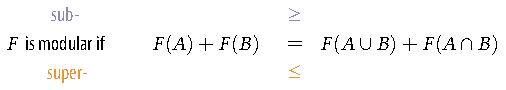
\includegraphics[width=3.9in]{figures/ineq_mod_2.pdf}}%

\uncover<4->{%
\vspace{1em}
``Distance" from modularity
\begin{align*}
\zeta_F \defeq \max_{A, B \subseteq V} \big|F(A) + F(B) - F(A \cup B) - F(A \cap B)\big|
\end{align*}
}

\uncover<5>{%
\qtheorem{1}{
For any sub- or supermodular set function $F$, the mixing time of the Gibbs sampler is
\begin{align*}
t_{\textrm{mix}}(\epsilon) = \mathcal{O}\left(n^2 \exp(\zeta_F)\log\epsilon^{-1}\right).
\end{align*}
}}
\end{frame}


\begin{frame}{Improved Mixing using Semigradients}
\centering
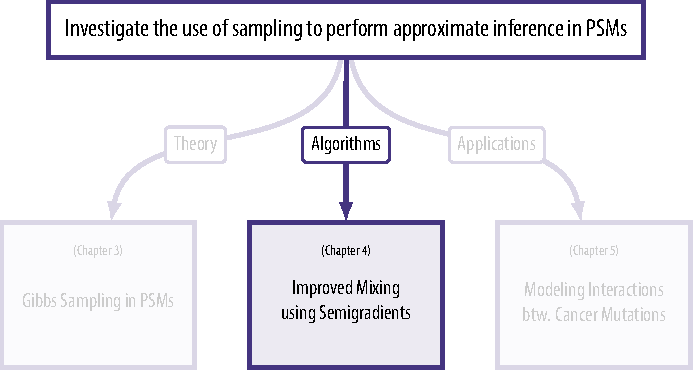
\includegraphics[width=\textwidth]{figures/chapters2.pdf}
\end{frame}

\begin{frame}{Bottlenecks}
\vspace{1em}
\centering
\only<1>{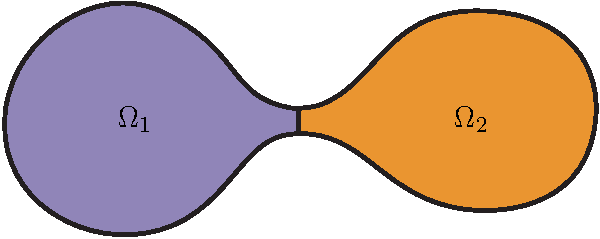
\includegraphics[width=0.9\textwidth]{figures/bottleneck1.pdf}}%
\only<2>{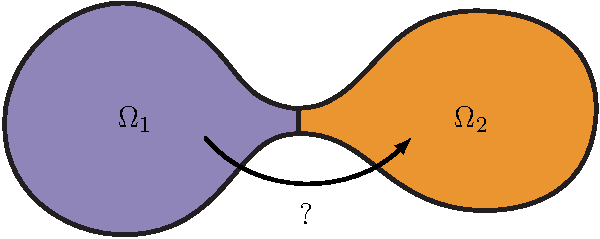
\includegraphics[width=0.9\textwidth]{figures/bottleneck2.pdf}}%
\only<3>{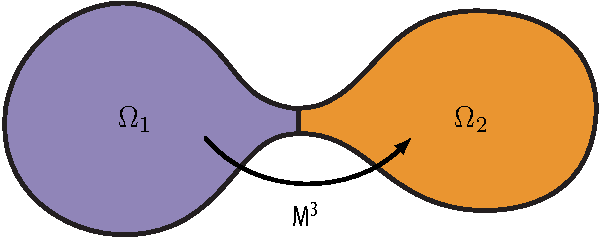
\includegraphics[width=0.9\textwidth]{figures/bottleneck3.pdf}}%
\end{frame}

\begin{frame}{Modeling Interactions between Cancer Mutations}
\centering
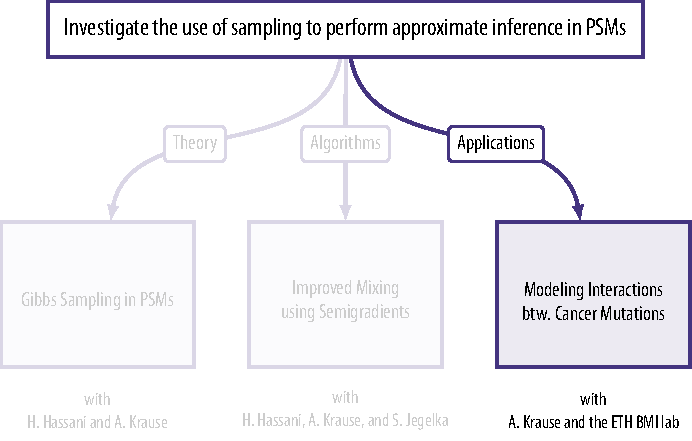
\includegraphics[width=\textwidth]{figures/chapters3.pdf}
\end{frame}

\begin{frame}{Approximate Maximum Likelihood Learning}
\vspace{-1em}
Data $\ \mathcal{D} = \{D_1,\ldots, D_N\}$

\uncover<2->{%
\only<1-2>{%
\vspace{3em}
\centering
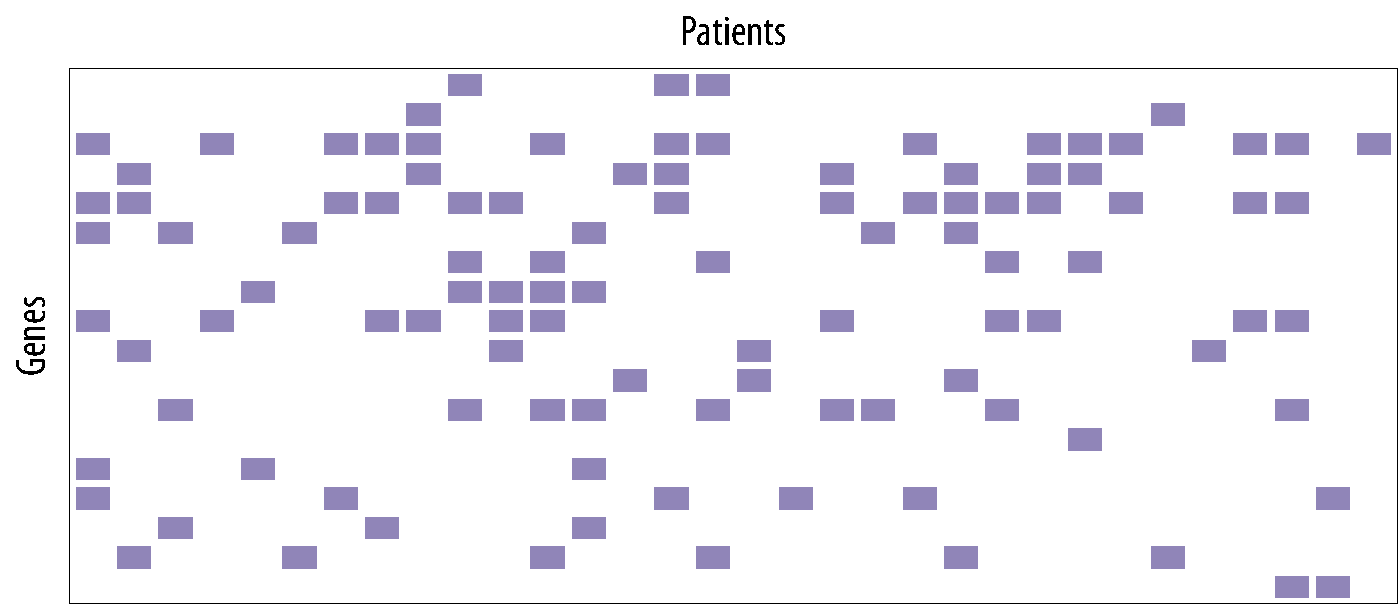
\includegraphics[width=3.7in]{figures/example1.pdf}
}%
\only<3->{%
\begin{align*}
\ell(\btheta) &= \sum_{i=1}^N F(D_i; \btheta) - N \log Z(\btheta)\\[1em]
\uncover<4->{\nabla_{\btheta} \ell(\btheta) &= \frac{1}{N}\sum_{i=1}^N \nabla_{\btheta} F(D_i; \btheta) - \alt<4>{}{\color{col2}}\mathbb{E}_{p}\left[ \nabla_{\btheta} F(S; \btheta)\right]\\[0.5em]}
\uncover<6->{&\approx \frac{1}{N}\sum_{i=1}^N \nabla_{\btheta} F(D_i; \btheta) - \color{col2}\frac{1}{M}\sum_{i=1}^M \nabla_{\btheta} F(S_i; \btheta)}
\end{align*}
}%
}
\end{frame}

\begin{frame}{The FLiD Model \qcitea{Tschiatscheck et al., 2016}}
$p(S) = \displaystyle\frac{1}{Z}\exp \big( F(S) \big)$\\[1em]
$F(S) = \displaystyle\sum_{i \in S} u_i + \displaystyle\sum_{j=1}^{L} \left(\displaystyle\max_{i \in S} w_{ij} - \displaystyle\sum_{i \in S} w_{ij}\right),\ \ \ u_i \in \mathbb{R}, w_{ij} \in \mathbb{R}_{\geq 0}$

\vspace{2em}
\uncover<2->{%
\begin{columns}
\begin{column}{0.5\textwidth}
\centering
\only<1-2>{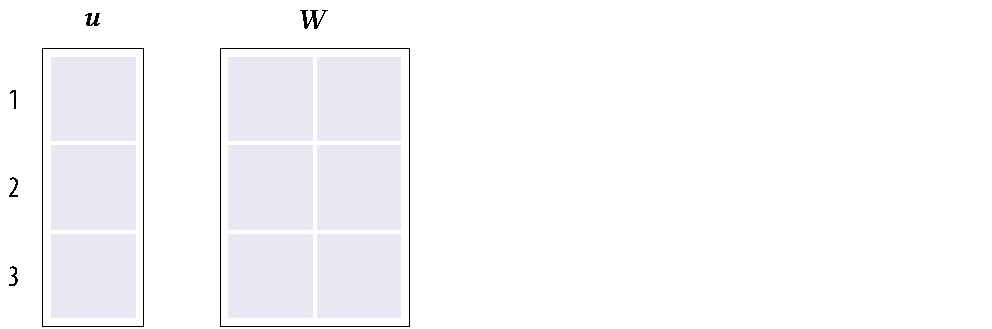
\includegraphics[height=1.4in]{figures/flid_empty.pdf}}%
\only<3>{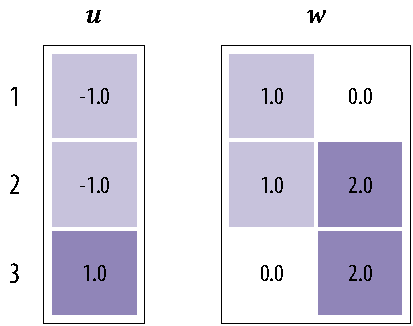
\includegraphics[height=1.4in]{figures/flid.pdf}}%
\only<4>{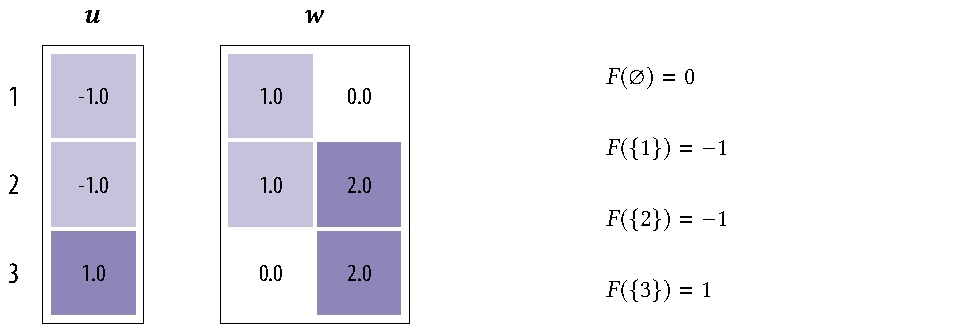
\includegraphics[height=1.4in]{figures/flid_numbers_1.pdf}}%
\only<5>{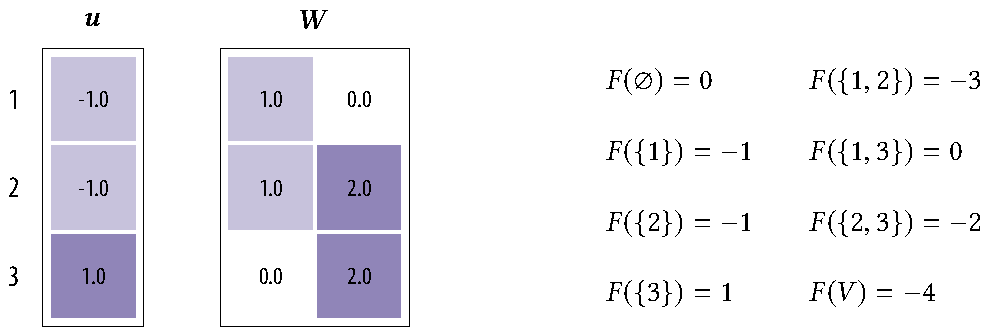
\includegraphics[height=1.4in]{figures/flid_numbers_2.pdf}}%
\only<6>{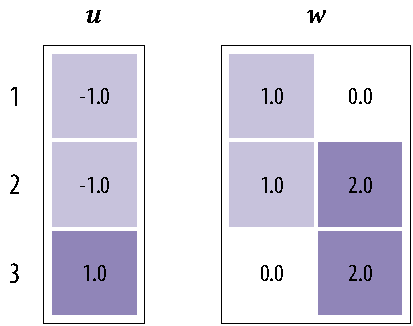
\includegraphics[height=1.4in]{figures/flid.pdf}}%
\end{column}
\begin{column}{0.5\textwidth}
\only<4-6>{

}
\only<6>{
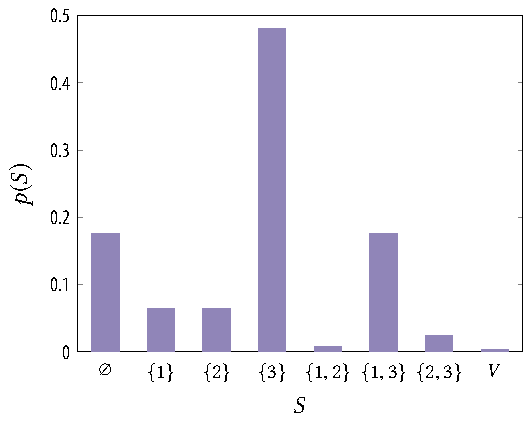
\includegraphics[height=1.5in]{figures/flid_dist.pdf}}%
\vspace{-2.1em}
\end{column}
\end{columns}%
}
\end{frame}


\begin{frame}{Synthetic Data}
\begin{columns}
\begin{column}{0.3\textwidth}
\only<1>{\hspace{3em}$n_{\mathrm{iter}} = 0$}%
\only<2>{\hspace{3em}$n_{\mathrm{iter}} = 100$}%
\only<3>{\hspace{3em}$n_{\mathrm{iter}} = 200$}%
\only<4>{\hspace{3em}$n_{\mathrm{iter}} = 300$}%
\only<5>{\hspace{3em}$n_{\mathrm{iter}} = 400$}%
\only<6>{\hspace{3em}$n_{\mathrm{iter}} = 500$}%
\only<7>{\hspace{3em}$n_{\mathrm{iter}} = 600$}%
\only<8>{\hspace{3em}$n_{\mathrm{iter}} = 700$}%
\only<9>{\hspace{3em}$n_{\mathrm{iter}} = 800$}%
\only<10>{\hspace{3em}$n_{\mathrm{iter}} = 900$}%
\only<11>{\hspace{3em}$n_{\mathrm{iter}} = 1000$}%
\end{column}
\begin{column}{0.7\textwidth}
\centering
\only<1>{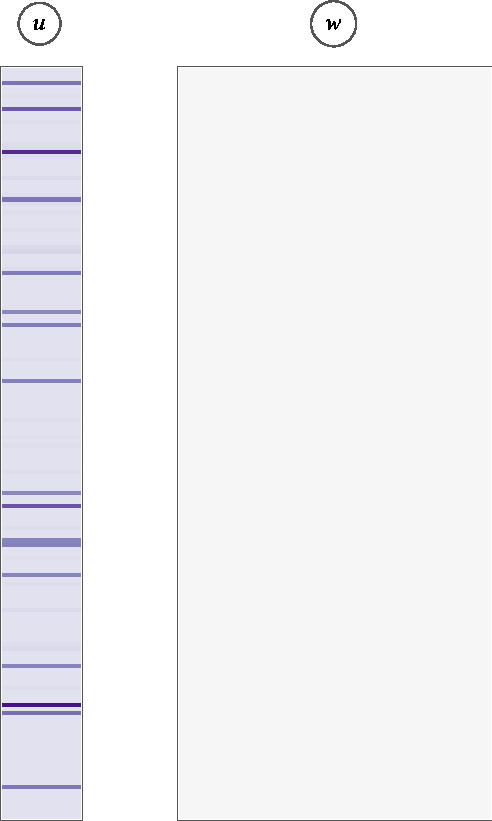
\includegraphics[height=0.9\textheight]{figures/mat_syn_0.pdf}}%
\only<2>{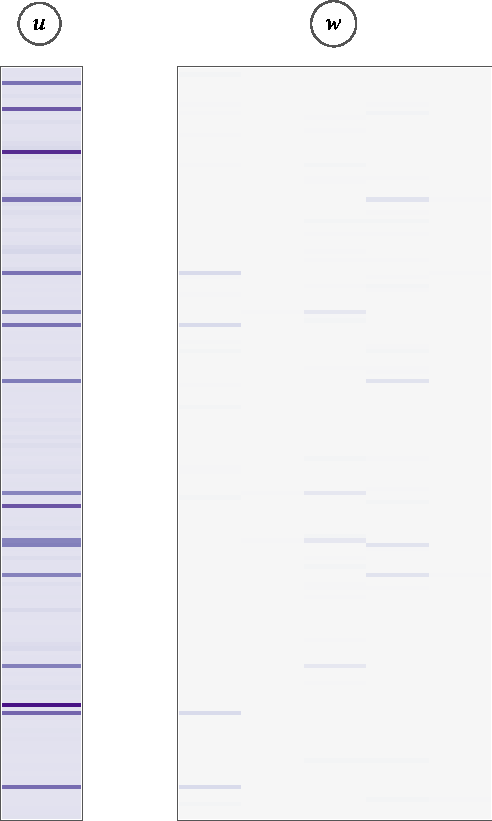
\includegraphics[height=0.9\textheight]{figures/mat_syn_100.pdf}}%
\only<3>{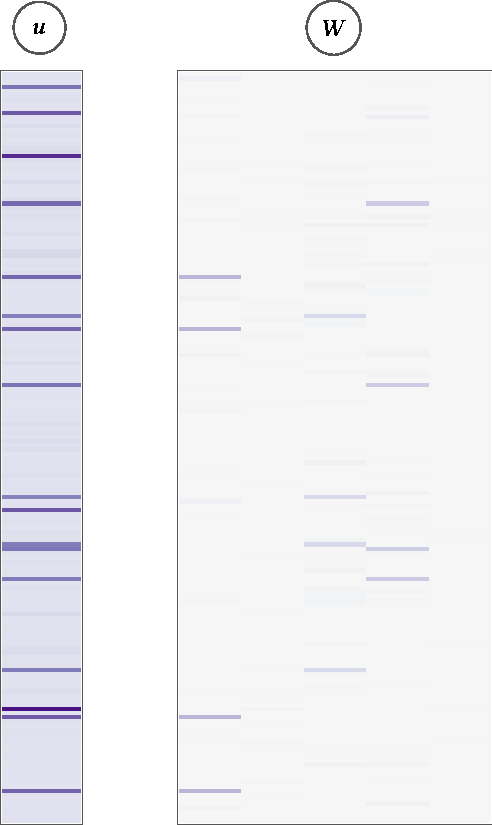
\includegraphics[height=0.9\textheight]{figures/mat_syn_200.pdf}}%
\only<4>{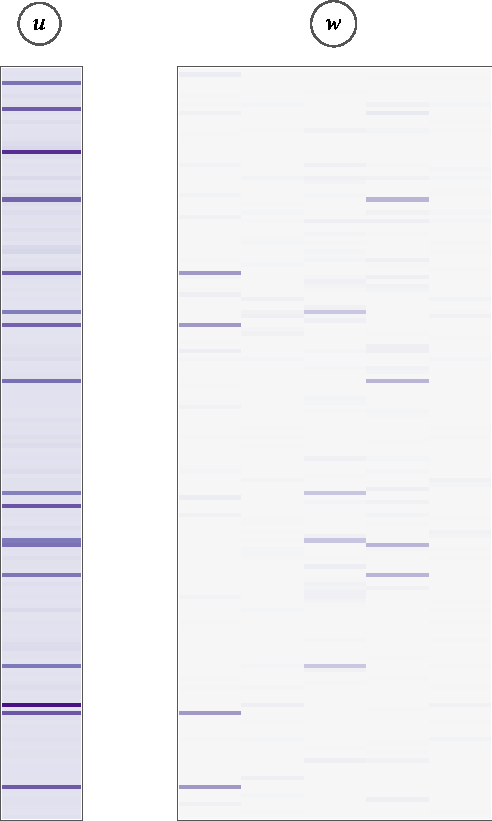
\includegraphics[height=0.9\textheight]{figures/mat_syn_300.pdf}}%
\only<5>{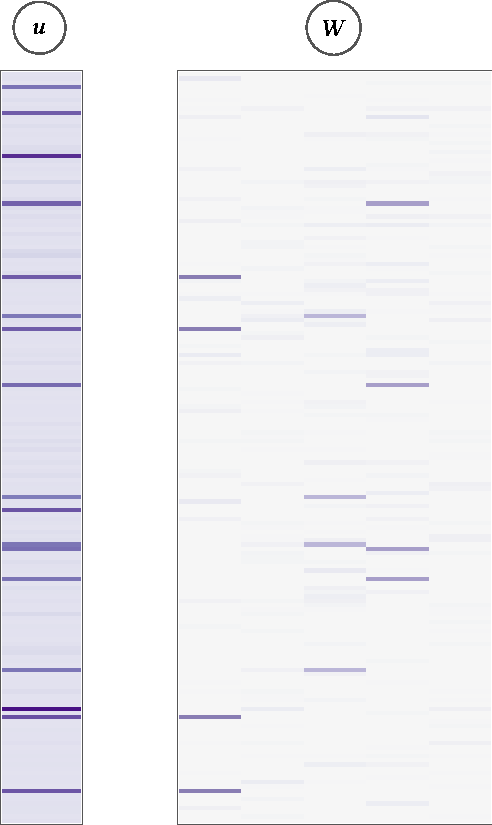
\includegraphics[height=0.9\textheight]{figures/mat_syn_400.pdf}}%
\only<6>{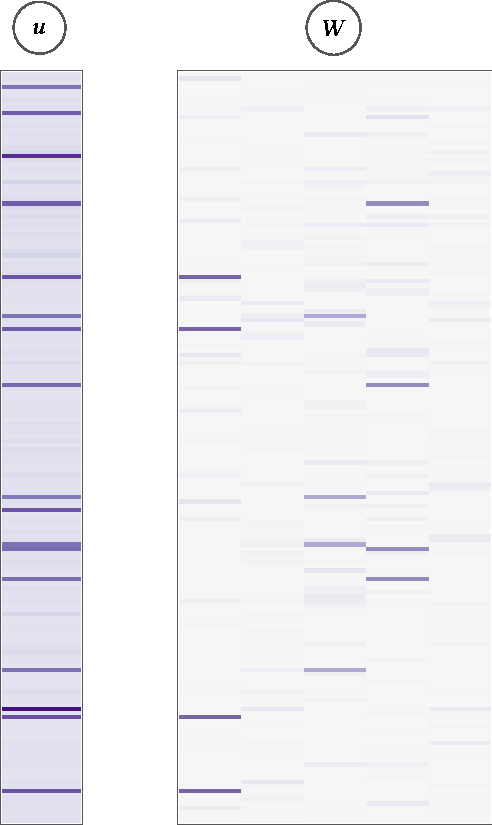
\includegraphics[height=0.9\textheight]{figures/mat_syn_500.pdf}}%
\only<7>{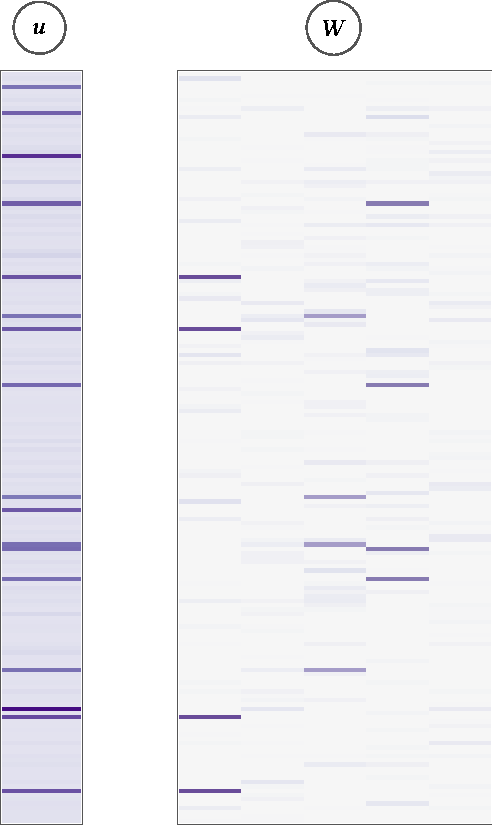
\includegraphics[height=0.9\textheight]{figures/mat_syn_600.pdf}}%
\only<8>{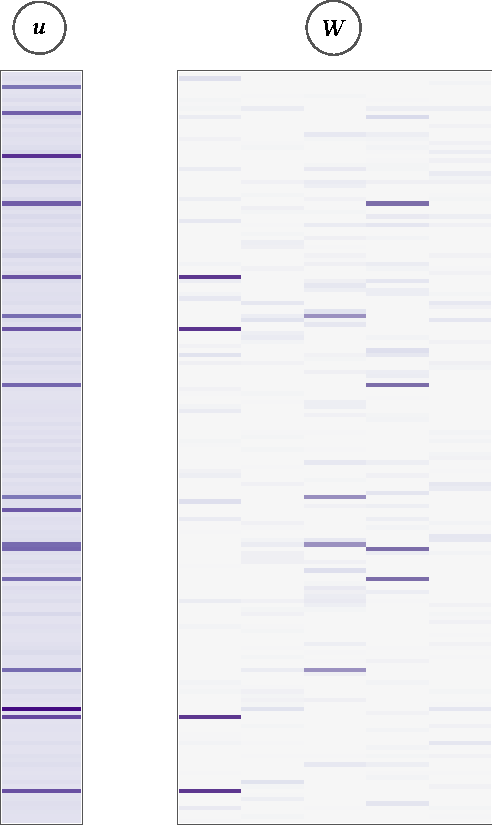
\includegraphics[height=0.9\textheight]{figures/mat_syn_700.pdf}}%
\only<9>{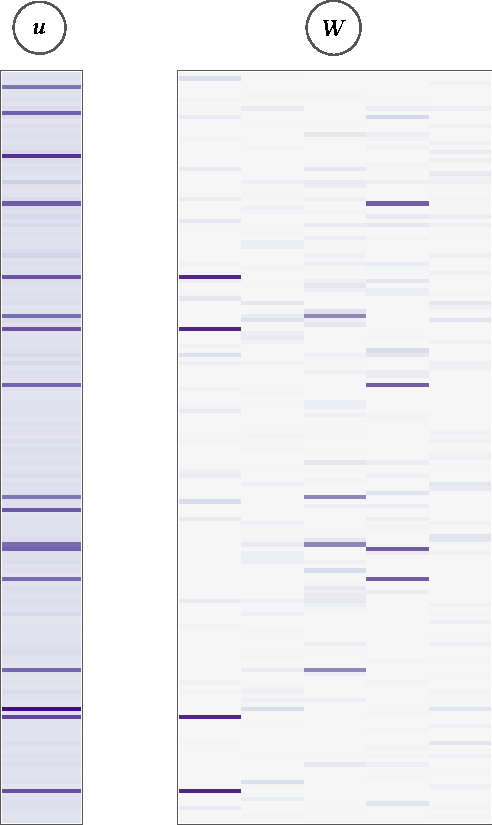
\includegraphics[height=0.9\textheight]{figures/mat_syn_800.pdf}}%
\only<10>{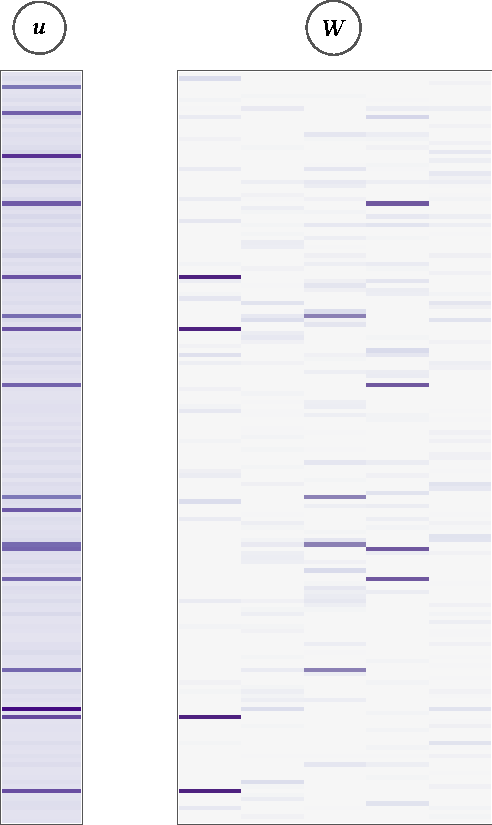
\includegraphics[height=0.9\textheight]{figures/mat_syn_900.pdf}}%
\only<11>{\includegraphics[height=0.9\textheight]{figures/mat_syn_1000.pdf}}%
\end{column}
\end{columns}
\end{frame}

\begin{frame}{Pipeline}
	\begin{enumerate}
		\item Learn model parameters $\*u, \*w$ from data\\[1em]
		\item Threshold $\*w$ to obtain candidate groups\\[1em]
		\item Apply statistical tests to assess mutual exclusivity\\[1em]
		\item Filter groups via online FDR control
	\end{enumerate}
\end{frame}

\begin{frame}{Synthetic Data}
$t\ $ groups of $k\ $ elements\\
\vspace{1em}
\centering
\includegraphics[width=0.93\textwidth]{figures/syn_multi.pdf}%
\end{frame}

\begin{frame}{Real Cancer Data (TCGA AML)}
\centering
\only<1>{\includegraphics[height=0.92\textheight]{figures/mat_aml.pdf}}%
\only<2>{\includegraphics[height=0.92\textheight]{figures/mat_aml_annotated.pdf}}
\end{frame}

\begin{frame}{Real Cancer Data (TCGA AML)}
\vspace{1em}
\centering
\includegraphics[width=0.85\textwidth]{figures/aml_1.pdf}\\[2em]
\includegraphics[width=0.85\textwidth]{figures/aml_2.pdf}
\end{frame}

\begin{frame}{Real Cancer Data (TCGA AML)}
\vspace{1em}
\centering
\includegraphics[width=0.85\textwidth]{figures/aml_3.pdf}\\[2em]
\includegraphics[width=0.85\textwidth]{figures/aml_4.pdf}
\end{frame}

\begin{frame}{Summary}
\vspace{1em}
\centering
\includegraphics[width=\textwidth]{figures/chapters_end.pdf}%
\end{frame}

\begin{frame}{Future Directions}
\begin{columns}
\begin{column}{0.6\textwidth}
\begin{itemize}
  \item<1-> Learn cancer type ``factorization"
  \vspace{3em}
  \item<4> Learn models that are guaranteed to mix fast
\end{itemize}
\end{column}
\begin{column}{0.4\textwidth}
\uncover<2->{%
\only<1-2>{\includegraphics[width=0.9\textwidth]{figures/flid_fact_1.pdf}}%
\only<3->{\includegraphics[width=0.9\textwidth]{figures/flid_fact_2.pdf}}%
}
\end{column}
\end{columns}

\end{frame}

\end{document}
